\raggedright
\mychapter{3}{Work Project 3}
	\label{ch:cc}
	\section{Esercizio 1: Logica Proposizionale}
		\label{sec:es1}
		Un agente intelligente che sfrutta tale approccio, si rifà al comportamento umano di ragionare su sue conoscenze personali. Quindi ha bisogno di una base di conoscenza in cui archiviare tutte queste informazioni, affinché possa usarle per trarne delle deduzioni.
		\par
		L'agente semplicemente ogni volta che ha bisogno di dedurre qualcosa, prima di tutto enuncia alla sua base di conoscenza qual'è la sua percezione in questo momento, dopodiché chiede a quest' ultima quale operazioni deve eseguire in base alla informazioni archiviate all' interno e comunica  di aver eseguito l' operazione. Ovviamente l' agente all' inizio non è a conoscenza di tutti i fatti che gli occorrono per completare la sua operazione, per tale ragione può raccogliere informazioni chiedendo i fatti(approccio dichiarativo) di cui gli interessa o in altri casi può avere già della conoscenza archiviata (approccio procedurale), di solito i due approcci vanno usati insieme per avere una buona base di conoscenza.
		\par
		Ovviamente tali informazioni non possono essere salvate nella conoscenza dell' agente in un linguaggio naturale o comunque in un qualsiasi modo in cui non sia possibile trarre delle conclusioni. Per tale motivo le frasi che definiscono la nostra conoscenza sono scritte con una certa sintassi, propria del linguaggio che vogliamo utilizzare, la stessa identica frase espressa naturalmente può essere tradotto in modi differenti in base alla diversa sintassi della logica che andiamo ad utilizzare. Però il risultato da ottenere sarà lo stesso che è indipendente dalla logica utilizzata, cioè avendo dei dati noti a priori, capire se si può riuscire a dedurre altre informazioni che a noi interessa sapere, tale relazione è detta di implicazione(entailment). Utilizzeremo la logica proposizionale, in cui la sintassi è composta da frasi atomiche, legate tra loro tramite connettivi logici per ottenere frasi più complesse, il singolo elemento della frase può assumere valore o vero o falso,infatti la semantica di tale logica è quella di trovare il valore vero di ogni frase dato la conoscenza nota a priori. Le operazioni tra i letterali sono: la negazione che muta il valore della nostro letterale, l' operazione di and che ci da vero solo se i due connettivi sono veri, or restituisce vero se uno dei due è vero, implicazione ci dà falso se dal vero deduciamo il falso e quella bicondizionale vera se e solo se entrambi i letterali hanno lo stesso significato.
		Per verificare la relazione di implicazione possiamo ricorrere a due strade la prima in cui enunciamo tutti i possibili mondi del nostro modello, per esempio tramite la tabella di verità,trovare quelli che rispettano la nostra base di conoscenza e la deduzione che stiamo facendo e se i mondi che rispecchiano la nostra percezione sono contenuti all' interno della concetto che vogliamo dedurre, allora possiamo dire che la nostra conoscenza implica quel fatto, sulla tabella li possiamo vedere facilmente osservando che quando sono veri i fatti allora anche ciò che vogliamo dedurre è vero.
		\par
		Questo metodo è molto oneroso quando i possibili mondi sono tanti ed enumerarli tutti sarebbe molto dispendioso sia in termini di spazio che di tempo, per tale ragione di preferiscono altre strade.
		\par
		Una possibile è scrivere le frasi in forma CNF e da li applicare metodi inferenziali per capire se la nostra conoscenza implica il fatto. 
		Prima di tutto però dobbiamo trasformare le frasi che abbiamo nella forma CNF, cioè or di congiunzioni atomiche, per farlo sfruttiamo le regole di equivalenza logica, purtroppo anche qui c'è un grande sforzo dell' essere umano che deve applicare tali regole affinché sia possibile dedurre qualcosa.
		Quando la nostra conoscenza è nella forma da noi voluta, possiamo provare a dimostrare che la nostra conoscenza con il negato della frase che vogliamo dedurre non sia soddisfacibile, cioè non esista nessun modello che implica quella frase, se ciò accade significa che la frase non negata è valida, cioè in tutti i mondi in cui è vera la nostra base di conoscenza è vera anche la frase, per verificare che not A sia soddisfacibile, basta prendere una coppia di clausole(congiunzione di letterali), presenti nella nostra base di conoscenza ed iniziare a derivare nuove informazioni,ciò avviene quando nella frase che si vengono a creare si presentino due letterali complementari (A e not A),
		applichiamo questo ragionamento ricorsivamente fino a che non riusciamo più a determinare nuove clausole e quindi quel fatto non è deducibile dalla nostra conoscenza, oppure se si arriva alla clausola nulla che ci permette di dire che la not A non è soddisfacibile allora A è valida.
		\par
		Tutti e due algoritmi sono completi e soundness.
		Un algoritmo è completo se é capace di enumerare tutte le relazione di implicazione possibili dalla base di conoscenza, ed è soundness perché ogni implicazione dell' algoritmo sono anche vere nel caso della base di conoscenza.
		Per entrambe le procedure enunciate vale il discorso che l' agente non conosce il significato della frase, quello è dato dall' essere umano, per l' agente una frase vale un' altra è solo capace di applicare le regole inferenziali
		\section{Esercizio 2: Reti Bayesiane}
		\label{sec:es2}
		L' approccio probabilistico, rispetto alle altre tipologie tiene conto di un grado di incertezza, a differenza per esempio di quello logico in cui un fatto può essere vero o falso, in questo caso si dice quanto quell' avvenimento è probabile, ma tale probabilità non ci dice a priori se sia vero oppure no, se per esempio affermo che oggi pioverà con una probabilità di 0.99 potrebbe capitare che non piova, proprio perché la probabilità definisce il livello di incertezza rispetto ad un conoscenza da noi acquisita e questa varia da persona a persona (agente ad agente), dipendete dal fatto che si possono avere esperienze diverse ed arrivare a valore di probabilità diverse.Le reti Bayesiane si rifanno al concetto di probabilità, più propriamente alla regola di Bayes: $P(causa|effetto)=\frac{P(effetto|causa)*P(causa)}{p(effetto)}$, una rete Bayesiana di solito è fatta in questo modo:
		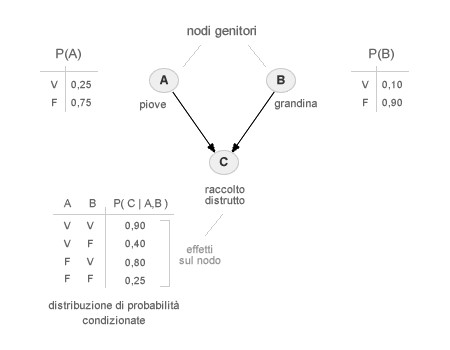
\includegraphics[width=0.95\textwidth, height=0.40\textheight]{retebayesiana.jpg}
		come osserviamo ci sono dei nodi che determinano la variabile di cui vogliamo tenere conto, a cui si assegnano anche i valori di probabilità a priori e i collegamenti che indicano la relazione di causalità tra i nodi, infatti la freccia che va da un nodo verso un altro determina tale relazione.
		\par 
		Per realizzare tale rete dobbiamo tenere conto delle relazioni di causalità delle nostre variabili, così facendo otteniamo una rete che riesce ad esplicare bene le nostre conoscenze ed è compatta, infatti qualsiasi altro modo di realizzare la rete ne aumenterebbe la complessità.Una rete così realizzata permette di effettuare calcolo delle probabilità in modo semplice, perché infatti in una rete del genere vale l' indipendenza condizionata, cioè una volta che io definisco un valore per una variabile padre le variabili figlio sono indipendenti tra di loro, quindi se per esempio la variabile A è padre di B e C la probabilità $P(B and C)=P(B|A)*P(C|A)$, altrimenti se non si avrebbe l' indipendenza non potremmo scrivere i due domini separati, quindi dovremmo tener conto anche della probabilità di B dato C. Per queste reti si ha anche il concetto di semantica locale, cioè ogni nodo è indipendente dai suoi non discendenti se viene dato il nodo padre; e della coperta di Markov, un nodo è indipendente da tutti se dato il nodo padre, i figli e i padri dei figli.
		\par  
		Per ricavare dati da queste reti date le probabilità a priori, possiamo semplicemente calcolare tutti i valori di probabilità a posteriori che ci occorrono, metodo complesso nel caso in cui la rete sia grande e il numero di possibili valori delle variabili è elevato, di solito si può ricorrere all' approccio frequentistico, cioè generiamo un token, quest' ultimo avrà una probabilità di ottenere il valore del nodo pari alla probabilità dei valori del nodo e si inizia a campionare la rete facendo scorrere il token su tutta la rete,fissando il valore dei nodi con quelli che risultano dal campionamento, la configurazione dei valori ricavati, una volta raggiunti il numero di risultati voluti, si divide il numero di configurazioni ottenute per il numero di campioni valutati, tale metodo per un alto numero di campioni deve tendere all' approccio di calcolare le probabilità a posteriori. Le reti bayesiano così costruite sono statiche perché non tengono conto di un riferimento temporale, infatti esistono le reti bayesiane dinamiche che tengono conto anche di un valore temporale suddiviso in istanti.Quindi la variabile casuale non ha solo relazioni con altre variabili, ma anche con se stessa però valutata in istanti diversi di tempo.I valori di probabilità di solito che vengono ricavate su tali reti sono: il filtering cioè la probabilità che avvenga un determinato fatto all' istante t dato i fatti precedenti e l' evidenza; lo smoothing la probabilità che un fatto in un istante t-k con k che va da 0 a t data l' evidenza fino all' istante t;
		la previsione, la probabilità di un fatto all' istante t+k con k>1 dato i fatti e l' evidenza fino a t;
		la spiegazione migliore, cioè data la probabilità all' istante t di fatti ed evidenza quali sono, quei determinati valori che ci permettono di avere quella probabilità.
		\par 
		Per esempio il filtering può essere facilmente calcolato ricorsivamente, infatti conosciuto il fatto iniziale ed essendo i processi stazionari, cioè per passare da un fatto ad un altro la tabella della probabilità non cambia, cioè la legge che prevede tale cambiamento è sempre la stessa, così facendo conoscendo lo stato iniziale posso successivamente determinare quello all' istante successivo e poi pesare la probabilità di quello stato data l' evidenza, esiste anche una tecnica detta di particle filtering in cui faccio un campionamento sul fatto iniziale, propago tali esempi sul campione successivo li peso per l' evidenza e rifaccio il campionamento per lo stato successivo tenendo conto del nuovo peso dei campioni, ovviamente per ottenere il valore di probabilità di una determinata configurazione, dobbiamo dividere il numero di casi uguali per il totale di campionamenti effettuati e per un alto valore di di quest' ultimi la mia probabilità tende a quella reale che avrei ottenuto con il filtering. Queste reti permettono anche di essere usate anche nel machine learning. Dato un insieme di ipotesi possiamo vedere qual' è la probabilità di una di queste data un evidenza cioè vogliamo calcolare la probabilità di $P(hi|d)$ dove hi è l' ipotesi e d è l' evidenza, ovviamente ad ogni nuovo valore potrebbe la hi che massimizza la probabilità cambia. Ovviamente non è molto agevola portare avanti i calcoli per tutte le ipotesi per tale ragione si sceglie quella che massimizza il valore a posteriori (MAP), cioè quella ipotesi che massimizza $\alpha*P(d|hi)*p(hi)$ dove $\alpha$ è il valore di normalizzazione, si può anche massimizzare il logaritmo di tale funzione, nel caso in cui le ipotesi hanno probabilità a priori (stessa complessità) uguali si può usare la maximum-likelihood (ML), in cui basta solo massimizzare $p(d|hi)$,ovviamente possiamo usare i logaritmi nel caso in cui compaiano esponenziali per rendere la massimizzazione della derivata molto più facile.
		
		\section{Esercizio 3: Reti Neurali}
			\label{sec: es3}
			Le reti neurali sono un meccanismo computazionale che si ispira al funzionamento del cervello umano. Sono rappresentabili tramite un grafo orientato, i cui nodi costituiscono un modello matematico del neurone ed ai cui archi orientati è associato un peso. Ogni nodo \textit{i} calcola la sua uscita $a_{i}$ applicando una funzione di attivazione \textit{g}, \texttt{activation function}, alla somma pesata degli ingressi, propagatisi dai nodi \textit{j} tramite l'arco corrispondente di peso $W_{i,j}$.
			\begin{equation}
			a_{i} = g(in_{i}) =g( \sum_{j=0}^n W_{j,i} a_{j})
			\end{equation}
			\medskip
			\begin{center}
				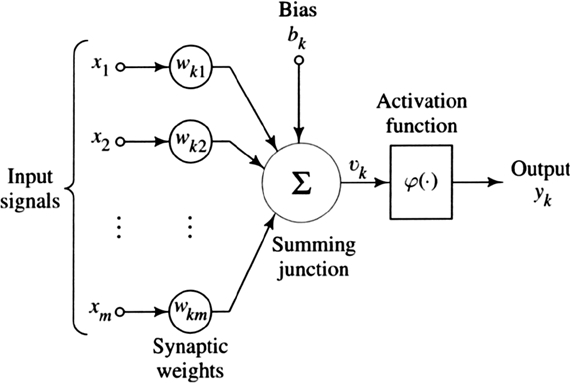
\includegraphics[width=0.8\textwidth, height=0.3\textheight]{neurone.jpg}
			\end{center}
			La funzione di attivazione storicamente utilizzata era quella di \emph{soglia}; in seguito si è diffusa la funzione \emph{sigmoide}, continua e derivabile rispetto alla precedente.\par
			Possiamo classificare strutturalmente le reti neurali distinguendo le \texttt{Recurrent Networks} e le \texttt{Feed-Forward Networks}. Le ultime non si fondano sul concetto di stato interno, a differenza delle prime,queste possono essere suddivise in più livelli, o \emph{layers}. Le reti neurali a singolo layer riescono a rappresentare solo operazioni \emph{linearmente separabili}, a due tutte le funzioni continue e quelle a tre le discontinue.
			\begin{center}
				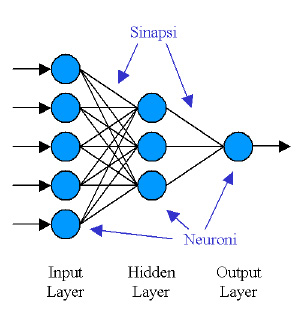
\includegraphics[scale=0.6]{RN-multilayer.jpg}
			\end{center}
			\par
			Una difficoltà non trascurabile risiede nella costruzione della struttura della rete neurale. Esse infatti sono sistemi \texttt{black-box}, il cui funzionamento interno è di difficile interpretazione logica, anche se è possibile avere un' interpretazione matematica che non ci aiuta nella costruzione.\par
			Per determinare il peso degli archi si utilizza l'algoritmo di \texttt{Back-Propagation}. Si considera una coppia ingresso-uscita del data-set e si costituisce una rete con pesi casuali(o uniformi per abolire l' onere computazionale). L'errore tra l'uscita ottenuta e quella desiderata verrà propagato all'indietro,per ogni  livello, così da modificare i pesi ed ottenere una migliore approssimazione. Inoltre si fa uso del \texttt{learning rate} per far si che la propagazione di un singolo esempio non influisca interamente sui valori dei pesi, altrimenti questi tenderebbero ad oscillare di molto se ogni esempio ci fornisce un alto valore di errore. La procedura viene iterata per ogni esempio, ciascuno dei quali consentirà una correzione dei pesi delineando una struttura della rete coerente con la funzione da approssimare. I problemi principali che riscontriamo in questo algoritmo sono l'eccessiva complessità temporale e la possibilità di arresto su di un minimo locale.\par
			Per quanto riguarda, invece,la determinazione del numero di neuroni, si procede tipicamente con un approccio \texttt{trial and error}, perché come già detto non si capisce qual' è il significato della rete, per tale motivo si parte da reti semplici, se queste dopo la \texttt{Back-Propagation} funzionano bene, le si usa, altrimenti di iniziano a inserire nuovi neuroni o layer di questi e si continua a testare la validità delle nuove reti create.\par
			In definitiva, le reti neurali si sono rivelate empiricamente un buon approssimatore di funzioni ed oggi il loro utilizzo ha ripreso vigore nella forma di \texttt{Deep Learning}. Ottengono, ad esempio, un basso \emph{error rate} nei problemi relativi al riconoscimento di caratteri e sono largamente diffuse nei sistemi multimediali per quanto concerne il riconoscimento di immagini, audio o nella \texttt{Computer Vision} in generale. Seppur presenti buoni risultati, bisogna ricordare che \emph{non esiste un algoritmo di apprendimento migliore in assoluto, ma bisogna trovare quello più adatto al problema dato.}
			
		\section{Esercizio 4: Cloud e Crowdsourcing}
			\label{sec:es4}
			Il \texttt{Cloud Computing} ed il \texttt{Crowdsourcing} sono paradigmi affermatisi nel nuovo millennio, figli della dirompete rivoluzione della rete non solo al livello culturale, ma anche economico, fornendo nuovi modelli per sviluppare ed offrire servizi al cliente.\par
			Il cloud prevede l'erogazione di risorse informatiche \emph{on demand} attraverso Internet. Tipicamente, in linea del tutto generale, un \texttt{Cloud Provider} fornisce un \emph{pool} condiviso di risorse; esse possono essere configurate da un cliente amministratore che le carica di valore aggiunto; infine il cliente finale usufruisce delle risorse in tal modo configurate per poi rilasciarle al termine del suo utilizzo.\par
			Il crowdsourcing è lo sviluppo collettivo di un progetto da parte di volontari esterni al suo ideatore. Questo fenomeno deriva dalla nascita delle prime \emph{open community} di condivisione, profondamente legato al concetto di \emph{sharing} portato dalla rete  in tutti i campi. La \emph{community open source} è stata la prima a sfruttare i benefici del crowdsourcing, ma questo paradigma si è diffuso anche in ambito aziendale con il modello di business di \emph{open enterprise}.\par
			Quantopian applica questi concetti fornendo i servizi per scrivere algoritmi di trading e rendendoli disponibili all'intera community, nella quale si potranno condividere idee, codice e dati. Esso, inoltre, investe un capitale sugli algoritmi con le migliori performance, condividendo i profitti con l'autore. Rappresenta, dunque, un modello di business all'avanguardia, che sfrutta pienamente le potenzialità della community, guidandola tramite i propri strumenti e ricavando introiti dall'impulso creativo a cui il crowdsourcing porta.
			\par 
			Tale piattaforma offre molti dataset direttamente senza importarli da altre fonti o di dover andare alla ricerca compulsiva sul web. Nel nostro esempio vediamo operazioni di trading sulle azioni americane, di una nostra possibile società che ha un certo numero di azioni iniziali e decide quando vendere o comprare tali titoli per aumentare i suoi introiti partendo da un capitale iniziale ed osservando cosa accade in un determinato lasso di tempo.
			\par 
			Il codice fornisce tale output:
			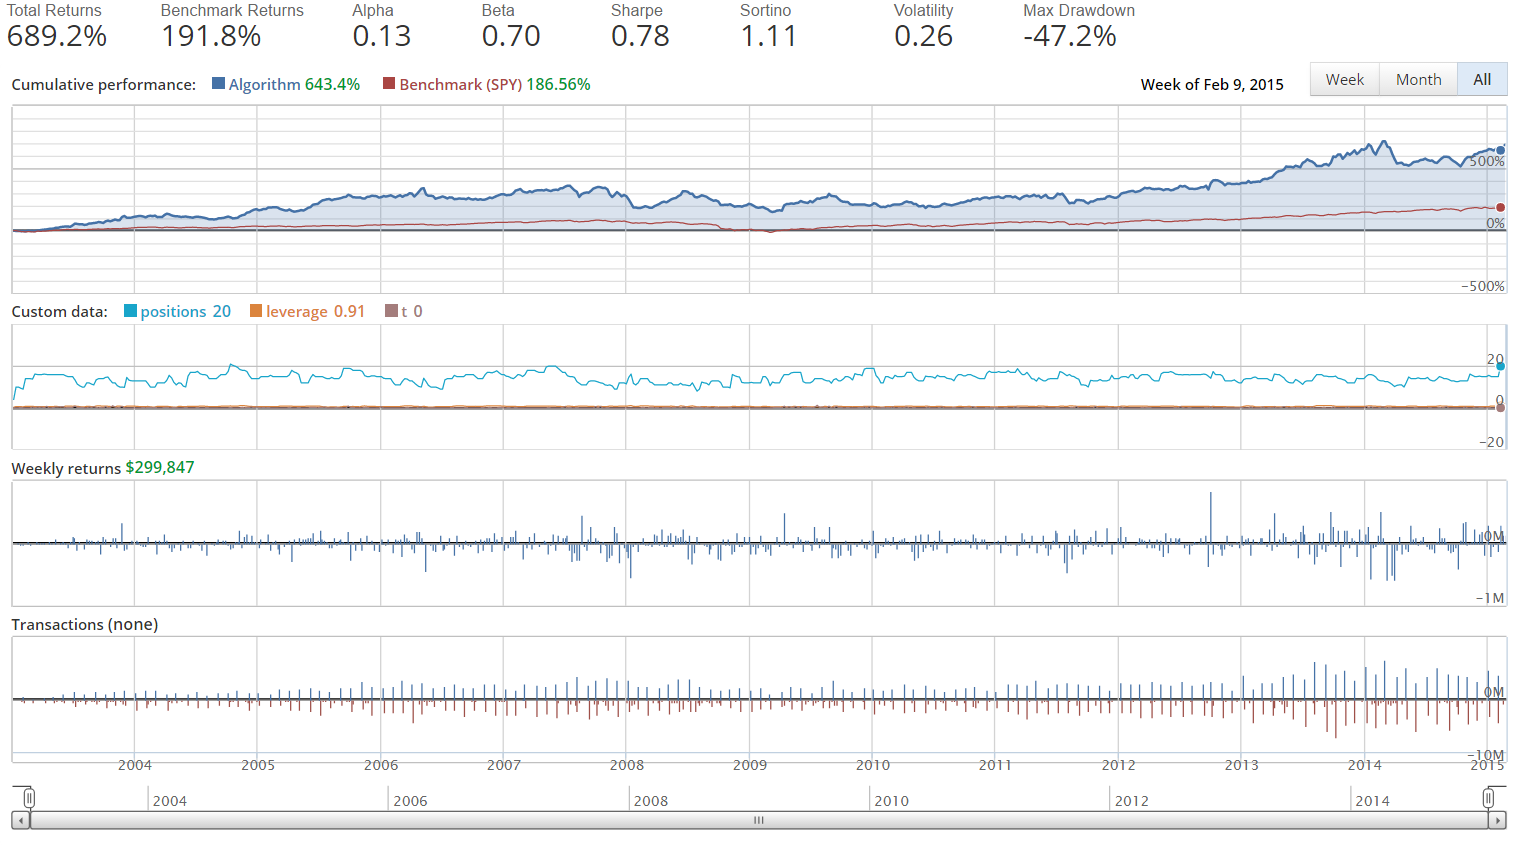
\includegraphics[width=1.0\textwidth, height=0.40\textheight]{inizio.png} 
			la linea rossa definisce il reale valore che si avrebbe avuto confrontandosi con il mercato, invece quello blu l' algoritmo quanto abbia stimato, il valore position ci dice il numero di azioni attive, cioè non ancora chiuse, leaverage ci dice quanto siamo disposti ad investire in base agli introiti,% t non ho capito
			il guadagno settimanale e la transazione monetaria che ci è stata.
			Come si può vedere dall' esempio la nostra scelte di trading secondo il nostro algoritmo è molto ottimistica rispetto a ciò che è successo realmente, anche se a grandi linea comunque rispetta ciò che è successo, dandoci però un guadagno falsato.
			La modifica dell' algoritmo, oltre ad essere permessa da qualsiasi pc essendo tutto in cloud, viene eseguita da una server farm che sicuramente è molto più performante del nostro pc infatti quello che si vede in figura solo le valutazioni del mercato americano in circa 12 anni, un onere di computazione non banale.
			Una possibile modifica dell' algoritmo è  puntare solo sulle azioni che ci danno un valore di utile, maggiore:
			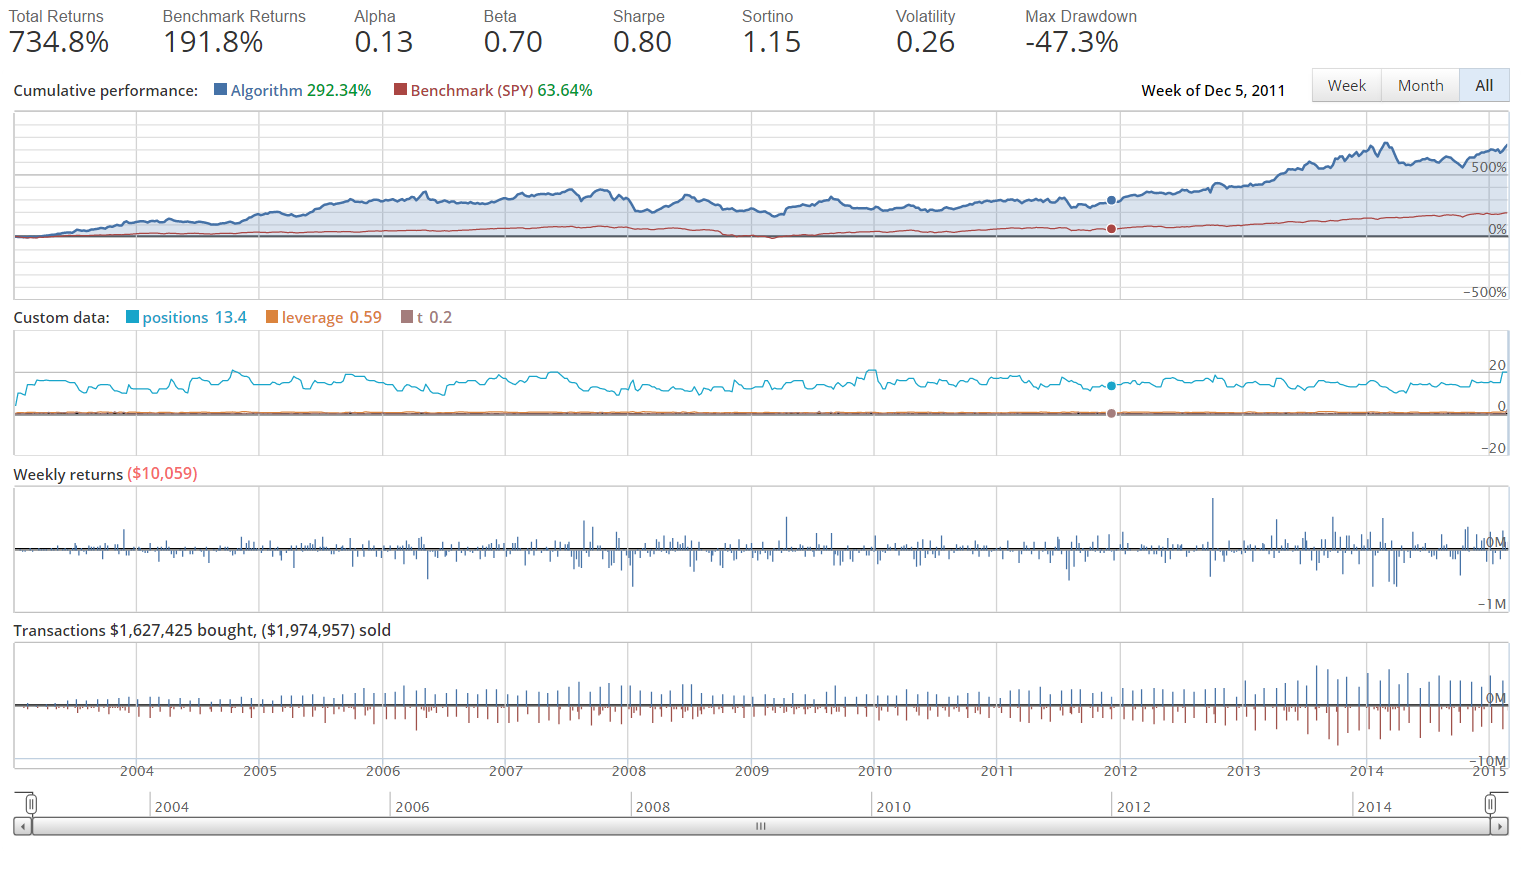
\includegraphics[width=1.0\textwidth, height=0.40\textheight]{factorfilter0,1.png} 
			Come vediamo l' algoritmo si è comportato meglio, perché ho preso solo le 3000 azioni che mi davano un' utilità sperata maggiore, quindi ho fatto trading su azioni che mi permettono di massimizzare i guadagni, ovviamente è un operazione che va bene a lungo termine, perché altrimenti non è detto che quell' azione abbia il comportamento sperato, può darsi che la sua efficienza sia minore, dato che fattori non ancora accaduti potrebbe in realtà portare ad un' utilità diversa.
			Un altro esperimento è stato quello di aumentare il profitto che si voleva fare con una determinata azione, tendendo quindi a cercare di sfruttare quando più quell' azione per massimizzare i guadagni,il risultato però è stato peggiore:
			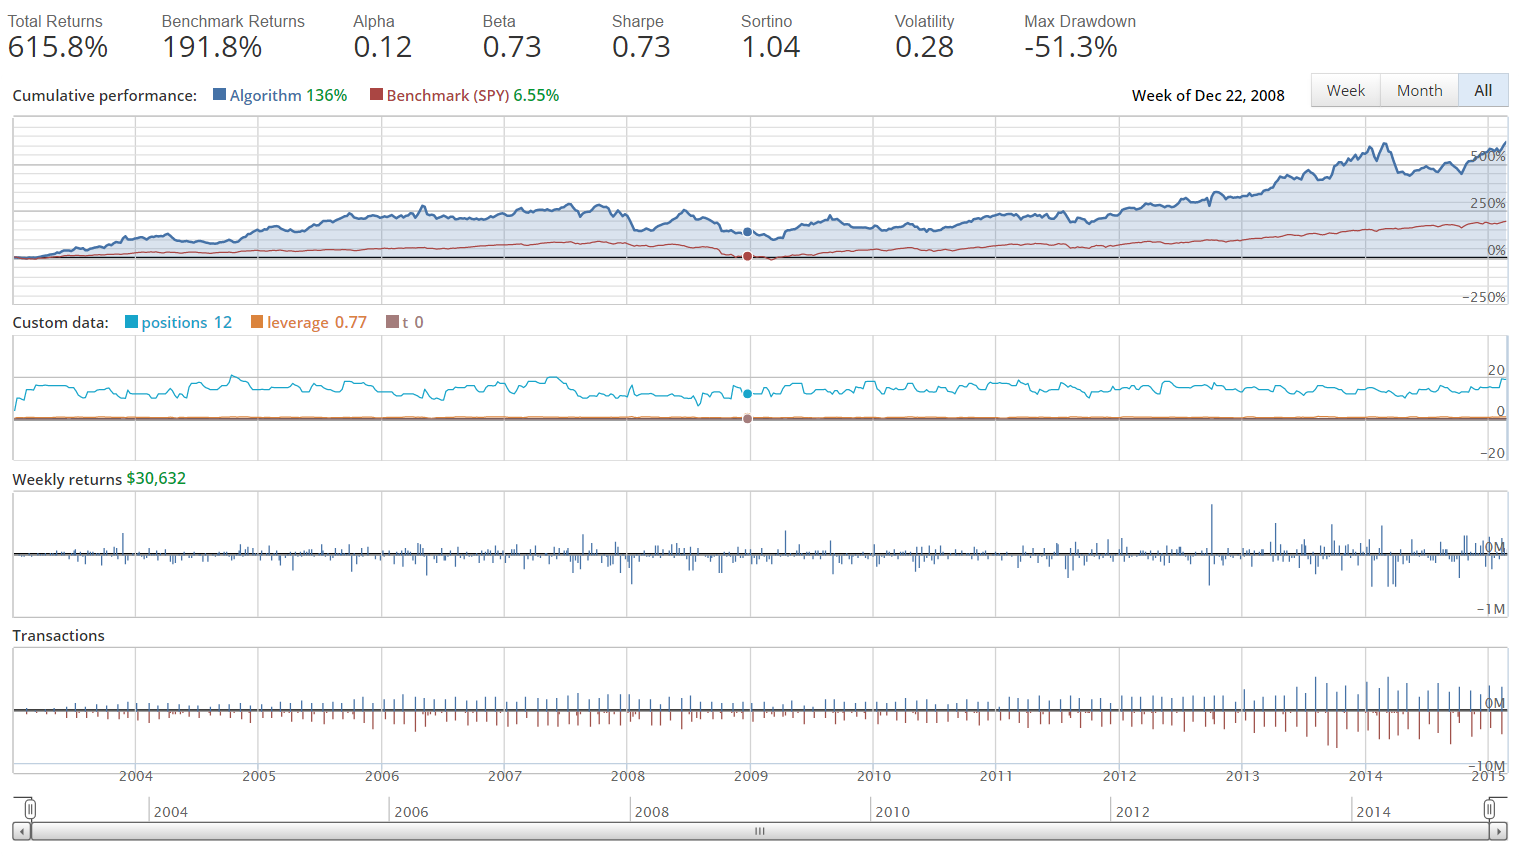
\includegraphics[width=1.0\textwidth, height=0.40\textheight]{stock2.png} 
			Possiamo vedere che il numero di transazioni sono state minori rispetto ai due casi precedenti, appunto perché una volta che si è iniziato a fare un trade su quell' azione fino a che non ci porta al guadagno voluto o scende al di sotto di un valore minimo non la vendiamo, così abbiamo cercato di attuare una politica più conservativa sulla compravendita, che ci ha portato a dei ricavi minori, ma ad un atteggiamento più consono a quello che in realtà è successo.